\documentclass{article}
\usepackage[utf8]{inputenc}
\usepackage{amsmath}
\usepackage{amsfonts}
\usepackage{amsthm}
\usepackage{parskip}
\setlength{\parindent}{0em}
\setlength{\parskip}{1em}
\usepackage{datetime}
\usepackage{algorithm}
\usepackage{algpseudocode}
\usepackage{booktabs}
\usepackage{hyperref}
\usepackage{enumerate}% http://ctan.org/pkg/enumerate
\usepackage{graphicx}
\usepackage[
	citestyle=ieee, 
    bibstyle=ieee,
    style=numeric-comp,
    sorting=nty,
    maxbibnames=99, % Make sure we are printing all authors in the appendix
]{biblatex}
\addbibresource{references.bib}
\usepackage{caption}
\usepackage{subcaption}
\usepackage{multicol}
\usepackage{pgffor} % Allows using foreach
\usepackage[section]{placeins} % Avoids placing floats before section
\usepackage[left=2.5cm, right=2.5cm]{geometry}

\newdateformat{monthyeardate}{%
  \monthname[\THEMONTH], \THEYEAR}

\title{Complex and Social Networks \\ Assignment 4 - Non-linear regression on dependency trees}
\author{Daniel Benedí García\\ Fernando Martín Canfrán}
\date{\monthyeardate\today}

\begin{document}
\maketitle
\begin{multicols}{2}
\tableofcontents
\end{multicols}

\section{Introduction}
\label{sec:introduction}
Centrality measures play a pivotal role in network analysis, as they help identify the most influential and well-connected nodes. Closeness centrality, in particular, offers a unique perspective by quantifying how easily information can flow from a node to all other nodes in the network. Its application to syntactic dependency networks (SDN) allows the study of the significance of words in conveying information, their role in sentence comprehension, and their impact on language processing and generation. See a representation of a SDN in Figure \ref{fig:sdn}.

To facilitate the computation of closeness centrality in SDN, this paper introduces the utilization of two distinct models based on two hypohteses. 
\begin{enumerate}[I]
    \item The measure of closeness centrality in syntactic dependency networks is significantly modeled by binomial (Erdos-Renyi) graphs, keeping the original numbers of edges and vertices.
    \item The measure of closeness centrality in syntactic dependency networks is significantly modeled by randomized graphs preserving the original degree sequence. The model depends on the original list of edges and a parameter $Q$ governing the repetitions of the random graph generation.
\end{enumerate}

These models offer a more efficient computational approach to evaluating closeness centrality while preserving the essential structural characteristics of the original networks.

The report studies the significance of the closeness centrality metrics obtained through these models in comparison to the original syntactic dependency networks. We seek to analyze how the metrics derived from the binomial (I) and degree-preserving random graph (II) models compare to those from the original networks. By doing so, we aim to tackle whether these simplified representations offer meaningful insights and faithfully capture the centrality of words in sentence structures.

This document is strucutred in four different sections. Next, results are presented in section \ref{sec:results}. Discussion and conclusions are covered in section \ref{sec:discussion}, and finally, some aspects of the methodology are presented in section \ref{sec:methods}.

\begin{figure}
    \centering
    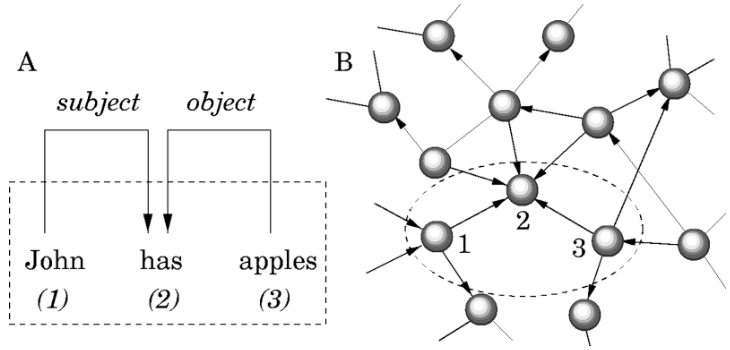
\includegraphics[width=0.5\textwidth]{figures/sdn.png}
    \caption{(a) The syntactic structure of a simple sentence. Here words define the nodes in a graph and the binary relations (arcs) represent syntactic dependencies. Here we assume arcs go from modifier to its head. The proper noun “John” and the verb “has” are syntactically dependent in the sentence. John is a modifier of the verb has, which is its head. Similarly, the action of has is modified by its object “apples.” (b) Mapping the syntactic dependency structure of the sentence in (a) into a global syntactic dependency network. Extracted from \cite{i2004patterns}}
    \label{fig:sdn}
\end{figure}

\section{Results}
\label{sec:results}
Tables \ref{tab:sig_karate}, \ref{tab:sig_barabasi_albert},  \ref{tab:sig_enron} and \ref{tab:sig_dblp} show the significance metrics computed for the different networks using \verb|evaluate_significance| provided by the \verb|clusterAnalytics| R package. Tables \ref{tab:best_canonical} and \ref{tab:best_no_canonical} highlight which clustering algorithm performs best according to the different metrics. As can be seen, the best algorithm is highly dependent on the network itself.

Surprisingly, the known canonical clustering does not seem to outperform the best clustering algorithm in terms of the metrics considered for Barabási-Albert blocks.

Table \ref{tab:jaccard} shows the global Jaccard indices for each of the networks and algorithms. In case a canonical clustering was known, it was used as the baseline. For the Enron network, we compared the algorithms to clustering produced by the Label Propagation algorithm. In the case of DBLP we used Louvain as a benchmark. Note that the clustering algorithms use randomness in their decisions, so two computations of the same algorithm produced two different clusterings, which in turn lead to a Jaccard index lower than 1 for Louvain.


\begin{table}[ht]
\centering
\begin{tabular}{l|ll|ll}
\toprule
\textbf{Metric} & \multicolumn{2}{l|}{\textbf{Karate} }    & \multicolumn{2}{l}{\textbf{Barabasi Albert Blocks} }      \\ 
\hline
   & \multicolumn{1}{l|}{best} & second best &  \multicolumn{1}{l|}{best} & second best\\ \hline
   
  \big\uparrow Internal Density  & \multicolumn{1}{l|}{Edge Betweenness} & Walktrap &   \multicolumn{1}{l|}{Walktrap} & Spin Glass \\ 
 \big\uparrow Edges Inside  & \multicolumn{1}{l|}{ground truth} & Label Propagation + FG &  \multicolumn{1}{l|}{Label Propagation} & Edge Betweenness \\ 
 \big\uparrow Average Degree  &\multicolumn{1}{l|}{ground truth} & Label Propagation + FG & \multicolumn{1}{l|}{Label Propagation} & Louvain + SG\\ 
\hline
 \big\downarrow Expansion  & \multicolumn{1}{l|}{ground truth} & Label Propagation + FG &\multicolumn{1}{l|}{Label Propagation} & Louvain + SG\\ 
 \big\downarrow Cut Ratio  &  \multicolumn{1}{l|}{ground truth} & Label Propagation + FG & \multicolumn{1}{l|}{Louvain + SG + LP} & \\ 
\hline
 \big\downarrow Conductance  &  \multicolumn{1}{l|}{ground truth} & Label Propagation + FG & \multicolumn{1}{l|}{Label Propagation} & Lovain \\ 
 \big\downarrow Normalized Cut & \multicolumn{1}{l|}{ground truth} & Label Propagation + FG& \multicolumn{1}{l|}{Label Propagation} & Lovain + SG\\ 
 \big\downarrow Maximum ODF & \multicolumn{1}{l|}{ground truth} & Label Propagation + FG& \multicolumn{1}{l|}{Label Propagation} & Spin Glass\\ 
 \big\downarrow Average ODF  & \multicolumn{1}{l|}{ground truth} & Label Propagation + FG & \multicolumn{1}{l|}{Label Propagation} & Spin-Glass \\ 
   \hline
\end{tabular}
\caption{Best values for communities with ground truth}
\label{tab:best_canonical}
\end{table}


\begin{table}[ht]
\centering
\begin{tabular}{lll}
    \toprule
    \textbf{Metric} & \textbf{Enron} & DBLP \\
    \midrule
    \big\uparrow Internal Density & Edge Betweenness & Label Propagation\\
    \big\uparrow Edges Inside & Label Propagation & Spin-Glass \\
    \big\uparrow Average Degree & Label Propagation& Louvain \\
    \midrule
    \big\downarrow Expansion & Label Propagation & Louvain \\
    \big\downarrow Cut Ratio & Label Propagation & Louvain \\
    \midrule
    \big\downarrow Conductance & Label Propagation & Louvain \\
    \big\downarrow Normalized Cut & Label Propagation & Louvain \\
    \big\downarrow Maximum ODF & Label Propagation & Louvain    \\
    \big\downarrow Average ODF & Label Propagation & Louvain \\
   \bottomrule
\end{tabular}
\caption{Best values for communities without ground truth}
\label{tab:best_no_canonical}
\end{table}

% latex table generated in R 4.3.2 by xtable 1.8-4 package
% Wed Nov 22 15:27:58 2023
\begin{table}[ht]
\centering
\begin{tabular}{lrrrrrr}
  \hline
 & Louvain & Label Propagation & Walktrap & Edge Betweenness & Fast Greedy & Spin-Glass \\
  \hline
karate & 0.7977941 & 0.7977941 & 0.5853758 & 0.4040033 & 0.7977941 & 0.6147876 \\
  Barabasi-Albert & 0.8470966 & 0.2700000 & 0.7433218 & 0.8605959 & 0.8637888 & 0.8798209 \\
  ENRON & 0.1534839 & 1.0000000 & 0.2247313 & 0.1095882 & 0.4229562 & 0.1800507 \\
  DBLP & 0.7845611 & 0.2427005 & 0.2691897 & 0.5206746 & 0.6423933 & 0.3293205 \\
   \hline
\end{tabular}
\caption{Global jaccard indices for each data set and clustering algorithm}
\label{tab:jaccard}
\end{table}

% latex table generated in R 4.3.2 by xtable 1.8-4 package
% Wed Nov 22 15:27:58 2023
\begin{table}[ht]
\centering
\begin{tabular}{lllll}
  \hline
Network & Vertices & Edges & Mean.Degree & Density \\ 
  \hline
Karate & 34 & 78 & 4.5882 & 0.139 \\ 
  Barabasi-Albert & 200 & 800 & 8 & 0.0402 \\ 
  ENRON & 182 & 2097 & 23.044 & 0.1273 \\ 
  DBLP & 2130 & 4587 & 4.307 & 0.002 \\ 
   \hline
\end{tabular}
\caption{Summary of the properties of the networks used.}
\label{tab:summary}
\end{table}


\section{Discussion}
\label{sec:discussion}
\subsection{Scaling of vertex degree}

The traces of the evolution of the degree for different vertices, show that the evolution curve has the same shape independently of their arrival time. Indeed, looking at the plots from Appendix \ref{app:evolution}, we can observe that the growth function of a vertex does not depend on its arrival time.

Different growth models, however, present very different scaling curves, as noted in Section \ref{sec:results}. Table \ref{tab:fitted_evol} shows the specific parameters of all fitted curves. We only consider the case for the vertex arriving at time 1, since all other curves present an identical shape once they reach the same lifespan of any other vertex.

\begin{table}[!htb]
\centering
\begin{tabular}{ccccccccc}
                                                         & \multicolumn{8}{c}{\textbf{Growth Model}}                                           \\ \cline{2-9} 
                                                         & 0    & 1    & \multicolumn{2}{c}{2} & \multicolumn{2}{c}{3} & \multicolumn{2}{c}{4} \\
\textbf{Graph Model}                                     & $a$  & $a$  & $a$        & $b$      & $a$         & $c$     & $a$        & $d_1$    \\ \hline
\multicolumn{1}{r|}{Barabási-Albert}                     & 0    & 1.44 & 1.44       & 0.5      & 524.83      & 0       & 76.24      & -1.95    \\
\multicolumn{1}{r|}{Growth + Random Attachment}          & 0    & 0.05 & 10.43      & 0.09     & 30.11       & 0       & 2.67       & -1.56    \\
\multicolumn{1}{r|}{No Growth + Preferential Attachment} & 0.01 & 4.8  & 0.01       & 1        & 1046.12     & 0       & 241.88     & -1.96   
\end{tabular}

\vspace{1em}

\begin{tabular}{ccccccccccccc}
\multicolumn{2}{c}{0+} & \multicolumn{2}{c}{1+} & \multicolumn{3}{c}{2+} & \multicolumn{3}{c}{3+}     & \multicolumn{3}{c}{4+}         \\
$a$       & $d$        & $a$      & $d$         & $a$    & $b$  & $d$    & $a$      & $c$ & $d$       & $a$     & $d_1$    & $d_2$     \\ \hline
0         & 383.23     & 1.44     & 0           & 0.69   & 0.23 & -6.21  & 848.49   & 0   & -844.52   & 3.23    & 26430.96 & -34.85    \\
0         & 29.8       & 0.01     & 26.38       & 18.01  & 0.07 & -10.21 & 4815.89  & 0   & -4786.09  & 2.93    & 4.54     & -3.4      \\
0.01      & 0.74       & 7.2      & -1799.99    & 0.01   & 1    & -0.19  & 98626.47 & 0   & -98596.02 & 1506.69 & 60.81    & -16308.43
\end{tabular}

\caption{Values of fitted parameters per curve and graph model. Models 0 to 4 are shown above, and models 0+ to 4+ below.} \label{tab:fitted_evol}
\end{table}




Note that the mathematical expressions for each of the growth models are defined in Table \ref{tab:models_deg_evol}.

Through visual comparison against the raw data, most functions seem to fit the data well, as shown in the figures of Appendix \ref{app:sca_fit}, with the fitted function (green line) almost completely overlapping the data (black line) in all cases.

However, some of the results regarding which is the best model go against our intuition. It is especially the case for the \textit{No Growth + Preferential Attachment} model, whose scaling of vertex degree clearly follows a straight line. Models 0 and 0+ should be able to fit this data, and indeed, they visually do, so they should be preferred over the more complex Models 2 and 2+, when measuring the AIC. However, this is not the case and, aside from a possible mistake in our implementation which we have not been able to identify, our reasoning for this behaviour considers two possibilities:
\begin{enumerate}
    \item Although the data looks like a straight line, there might be some non-zero curvature that models 0 and 0+ are not able to capture, thus making their error be higher than it appears to be in plain sight.
    \item Since the number of data points is very large, the RSS values tend to be very large (and $n$ too), and even though the logarithm is considered for the computation of the AIC, RSS could still be the dominating factor, rendering $p$ (the sole advantage of models 0 and 0+ over 2 and 2+) insignificant, and making the decision of the best model be guided by random noise in the data.
\end{enumerate}

\subsection{Degree distribution}

The results of the fitted parameters can be seen in Table \ref{tab:fitted}.

\begin{table}[!htb]
\centering
\begin{tabular}{cccccccc}
\multicolumn{1}{r}{\textbf{}} & \multicolumn{5}{c}{\textbf{Probability Model}} \\ \cline{2-8} 
\multicolumn{1}{c}{\textbf{}} &
  \multicolumn{1}{c}{D. Poisson} &
  \multicolumn{1}{c}{D. Geom} &
  \multicolumn{1}{c}{Zeta} &
  \multicolumn{2}{c}{Truncated Z} &
  \multicolumn{2}{c}{Altmann} \\
\multicolumn{1}{c}{\textbf{Graph Model}} &
  \multicolumn{1}{c}{$\lambda$} &
  \multicolumn{1}{c}{$q$} &
  \multicolumn{1}{c}{$\gamma_1$} &
  \multicolumn{1}{c}{$\gamma_2$} &
  \multicolumn{1}{c}{$k_{max}$}  &
  \multicolumn{1}{c}{$\gamma_3$} &
  \multicolumn{1}{c}{$\delta$} \\ \midrule
\multicolumn{1}{r}{Barabási-Albert} & 5.98 & 0.17 & 1.49 & 0 & 7120 & 0 & 0.18 \\
\multicolumn{1}{r}{Growth + Random Attachment} & 6.99 & 0.14 & 1.42 & 0 & 70 & 0 & 0.15 \\
\multicolumn{1}{r}{No Growth + Preferential Attachment} & 6008 & 0 & 1.11 & 0 & 8401 & 0 & 0 \\
\bottomrule
\end{tabular}
\caption{Values of fitted parameters per distribution and graph model. Note that the model of a Zeta distribution with $\gamma = 3$ is not shown because no parameters were estimated.} \label{tab:fitted}
\end{table}

With these values, we are able to plot the probability distribution function of each probability model and compare it to the raw data.

However, through a visual representation of the fitted curves, as shown in Appendix \ref{app:degseq}, one can see that the curves do not model the data well. Note that the magnitude of the error is amplified by the representation in log-log scale (otherwise it is visually imperceptible), but it still shows that there has probably been a problem in the optimization procedure.

Indeed, for the \textit{Barabási-Albert} graph, one would expect to see the Zeta distribution model the data almost perfectly, since the curve with $\gamma = 3$ is visually identical to our data (and is also what the theoretical knowledge of the \textit{Barabási-Albert} model indicates). Instead, we see that it is somewhat displaced from the data and that the Zeta distribution with a variable $\gamma$ parameter does not converge to $\gamma=3$. Moreover, the geometric distribution, considered the best by AIC, is does not resemble the shape of the underlying data.

The distributions for the other two models show similar problems. For the \textit{Growth + Random Attachment}, the Poisson distribution is considered best. While it does show a downwards curve, as the data, it does not visually fit the underlying distribution. The \textit{No Growth + Preferential Attachment} model has a completely different shape, that our distributions are not able to fit; we would have expected the Poisson distribution to model this shape, but it is not the case.

\section{Methods}
\label{sec:methods}

Mean closeness cenrtality $\mathcal{C}$, as presented in \cite{newman2018networks}, is defined as follows:
\begin{align*}
 \mathcal{C} &= \dfrac{1}{N}\sum_{i=1}^N\mathcal{C}_i & \mathcal{C}_i &= \dfrac{1}{N-1}\sum_{\substack{j=1\\j\neq i}}^N \dfrac{1}{d_{ij}}& d_{ij} &=|P|
\end{align*}
Where $N$ is the number of nodes, $\mathcal{C}_i$ is the closeness centrality of vertex $i$, $d_{ij}$ is the geodesic distance between vertices $i$ and $j$, also as defined by \cite{newman2018networks}, and $P$ is the shortest path connecting edges $i$ and $j$ in the graph defined as a sequence (then $|P|$ is the length of said path).
\subsection{Description of the models}
\paragraph{Erdös-Rény model}
The Erdös-Rény model, also called binomial model, generates a random graph with a binomial process by flipping a coin and choosing whether an edge should be included or not. The used model is a slight variation of this one, because of instead of choosing the probability of an edge to be included or not, so the number of edges would follow a binomial distribution with expected value $\mathbb{E}[E] = p |E|$, the number of edges is fixed.
\paragraph{Switching model}
The switching model is a generator of random graphs given a degree sequence. This model has an interesting property to our experiments, because it preserve degrees although uniform sampling is not warranted.
\begin{algorithm}[!htb]
\caption{Switching mdodel}\label{algo:switching-model}
\begin{algorithmic}[line numbering]
\Require $G = (V,E), Q \in \mathbb{N}$
\For{$|E|\cdot Q$ times}
    \State $(u,v) \gets$ Choose u.a.r from $E$
    \State $(s,t) \gets$ Choose u.a.r from $E$
    \If{flip coin gets heads}
        \State Swap edges to $(u,t)$ and $(s,v)$
    \Else
        \State Swap edges to $(u,s)$ and $(v,t)$
    \EndIf
    \If{swap generates self-loops or parallel edges}
        \State Undo swap
    \EndIf
\EndFor
\end{algorithmic}
\end{algorithm}

The generation of graphs given a degree sequence yields multiple challenges adressed by some pieces in the literature \cite{blitzstein2011sequential, coolen2009constrained, milo2003uniform}. Our model deals with some of them, but to do so it lacks correctness in other areas. We believe this trade off is beneficial since the flawed properties of our implementation can be bounded. Some heuristics in our code are worth highlighting, referring to the Switching model:
\begin{itemize}
    \item Unbiased edge-picking. \\
    Asides from selecting a pair of edges to switch, we also check for possible switching randomly. Checking is referred not to the identification of failure switchings - those invalid because they don't preserve the degree sequence, but valid otherwise - but to the identification of switchings that pick the same edge to switch. Notice that since the graph is undirected, random selection of edges can yield a selected pair of edges $uv$,$vu$, where both $u,v\in V$ that are, in fact, the same edge. If this is not done, there is a bias because in our representation an edge is a pair of numbers in which the first one is smaller than the second. This bias causes that edges between nodes with smaller id or with high id are less probable.

    \item Guarantee of degree sequence preservation and impact on closeness centrality.\\
    The described implementation of the Switching model is flawed in the sense that it does not guarantee that no cycles are created. This can yield the generation of non-tree graphs, that although can otherwise show properties similar to those of SDN, fail to be acyclic as SDN are. This has a direct impact on the simulated closeness centrality. More detailed reasoning of this argument can be found in Appendix \ref{appendix:cc}.
\end{itemize}

\subsection{Implementation and execution}
The models have been implemented in C++ using the Boost Graph\footnote{See \url{https://www.boost.org/doc/libs/1_82_0/libs/graph/doc/index.html}} library \cite{siek2001boost}. We choose this library because it already implements some useful algorithms that we needed and also provides some representations for the graph. We used a adjacency list to represent the graph because the density is of edges (check table \ref{tab:1}) is low and this representation is really good for sparse graphs. In the switching model, we didn't used this representation because it does not allow to random access to the edges which is a frequent operation needed to this model. Therefore, we opted to use a \verb|std::vector| of pairs of integers to represent the edges and a \verb|std::set| of pairs in order to speed up the edge existence queries. 

Compilation flags include those recommended by the Boost library. Moreover, the repetitions of the trials for estimating the $p$-value has been parallelized using OpenMP allowing us to reduce the execution time of our experiments.

The experiments have been run with $Q = 1 +\log E$ for the switching model and the number of repetitions $T=100$ for all languages. Instead of computing bounds of the closeness centrality or its exact form, we opted to do a Montecarlo approximation with the 10\% of the nodes.

\subsection{Validation of the approximation of the closeness centrality \label{sub:validation}}
We chose to do an approximation of the closeness centrality by choosing a subset of the vertices and computing the closeness centrality between them. We decided that using the 10\% of the nodes to do this approximation was a reasonable amount in the trade-off between computational cost and approximation to the exact value.

In order to validate that our assumption was correct, we designed an experiment in which we run the method 100 times for the Catalan SDN, a binomial graph with the same number of vertices and edges as the Catalan SDN and applying the switching model $E \log E$ times to the Catalan SDN. Figure \ref{fig:validation} shows the results of the experiment in comparison with the exact computation of the metric. We observed that the approximations obtained are pretty close to the exact value, mainly for the binomial graph. The amount of error produced by this method can be observed in the third decimal and is evenly distributed above and below the real value, which allows us to conclude that the approximation is good enough to be used instead of the exact value.

\begin{figure}[!htb]
    \centering
    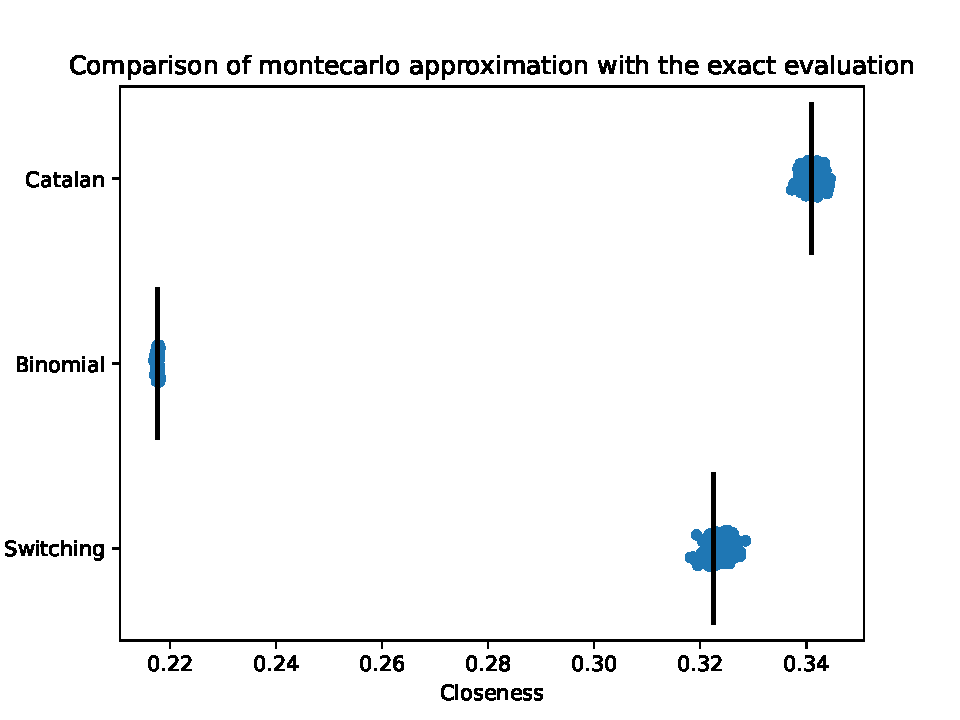
\includegraphics[width=0.75\textwidth]{figures/closeness_validation.pdf}
    \caption{Difference between the approximation and the exact value}
    \label{fig:validation}
\end{figure}

\addcontentsline{toc}{section}{References}
\printbibliography

\newpage
% Activate the appendix
% from now on sections are numerated with capital letters
\appendix
\def\Languages{
Arabic, Basque, Catalan,
Chinese, Czech, English,
Greek, Hungarian, Italian,
Turkish}

\section{Graphs of all the models for each language}\label{appendix:plots}

\foreach \lang in \Languages
{
\begin{figure}[!htb]
    \centering
    \includegraphics[width=0.7\textwidth]{figures/\lang_all_models.pdf}
    \caption{All models fitted for \lang}
\end{figure}
}
\pagebreak

\section{The best model by AIC for each language}\label{appendix:best-model-plots}

\foreach \lang in \Languages
{
\begin{figure}[!htb]
    \centering
    \includegraphics[width=0.7\textwidth]{figures/\lang_best_aic.pdf}
    \caption{The best model for \lang}
\end{figure}
}
\pagebreak

\section{The best model by $s$ for each language}

\foreach \lang in \Languages
{
\begin{figure}[!htb]
    \centering
    \includegraphics[width=0.7\textwidth]{figures/\lang_best_s.pdf}
    \caption{The best model for \lang}
\end{figure}
}
\pagebreak

\section{Data Samples provided for each language \label{appendix:data_samples}}
\foreach \lang in \Languages
{
\begin{figure}[!htb]
    \centering
    \includegraphics[width=0.7\textwidth]{figures/\lang_dataset.pdf}
    \caption{Data Samples for \lang}
\end{figure}
}
\pagebreak

\section{Weighted Nonlinear Least Squares \label{appendix:weighted}}

\foreach \lang in \Languages
{
\begin{figure}[!htb]
    \centering
    \begin{subfigure}{0.4\textwidth}
        \includegraphics[width=\textwidth]{figures/\lang_best_aic_weighted.pdf}
        \caption{Model with smallest AIC for \lang.}
    \end{subfigure} \hfill
    \begin{subfigure}{0.4\textwidth}
        \includegraphics[width=\textwidth]{figures/\lang_best_s_weighted.pdf}
        \caption{Models with smallest $s$ \lang.}
    \end{subfigure}
    \caption{Models fitted for language \lang}
\end{figure}
\begin{figure}[!htb]
    \centering
    \includegraphics[width=0.7\textwidth]{figures/\lang_all_models_weighted.pdf}
    \caption{All models for language \lang.}
\end{figure}
}

\begin{table}[!htb]
\centering
\resizebox{\columnwidth}{!}{
\begin{tabular}{llllllllllll}
Language & 0 & 1 & 2 & 3 & 4 & 5 & 1+ & 2+ & 3+ & 4+ & 5+ \\ \hline

 Arabic & 1090.844 & 235.935 & 235.521 & 275.158 & 268.201 & 224.634 & 236.397 & 231.094 & 274.438 & 266.068 & 241.632 \\
 Basque & 276.863 & 32.845 & 32.396 & 64.283 & 49.796 & 33.756 & 32.756 & 33.646 & 89.041 & 50.941 & 35.646 \\
 Catalan & 814.121 & 35.646 & 32.216 & 148.302 & 98.362 & 28.594 & 33.100 & 31.855 & 154.736 & 90.916 & 35.415 \\
 Chinese & 274.712 & 89.864 & 88.606 & 88.801 & 97.953 & 85.676 & 89.439 & 87.615 & 87.605 & 99.951 & 102.902 \\
 Czech & 723.596 & 428.590 & 421.061 & 424.942 & 439.635 & 416.160 & 426.906 & 411.535 & 413.922 & 440.122 & 418.808 \\
 English & 724.102 & 152.683 & 154.417 & 247.931 & 184.732 & 155.759 & 154.457 & 156.371 & 257.720 & 185.313 & 183.950 \\
 Greek & 711.355 & 156.227 & 155.661 & 193.590 & 173.208 & 156.703 & 156.055 & 156.800 & 205.467 & 173.253 & 158.695 \\
 Hungarian & 610.872 & 143.952 & 143.565 & 274.453 & 269.788 & 145.511 & 143.633 & 145.551 & 265.868 & 241.818 & 147.481 \\
 Italian & 705.677 & 134.719 & 128.651 & 173.938 & 160.282 & 122.408 & 130.492 & 124.636 & 175.543 & 161.160 & 124.370 \\
 Turkish & 412.776 & 20.871 & 19.327 & 96.241 & 49.615 & 20.250 & 19.339 & 21.317 & 110.629 & 50.554 & 17.680 \\
\end{tabular}}
\caption{Akaike information criterion (AIC) of each model \label{tab:aic}}
\end{table}

\begin{table}[!htb]
\centering
\resizebox{\columnwidth}{!}{
\begin{tabular}{llllllllllll}
Language & 0 & 1 & 2 & 3 & 4 & 5 & 1+ & 2+ & 3+ & 4+ & 5+ \\ \hline

 Arabic & 866.211 & 11.301 & 10.888 & 50.525 & 43.567 & 0.000 & 11.764 & 6.460 & 49.805 & 41.434 & 16.998 \\
 Basque & 244.467 & 0.449 & 0.000 & 31.887 & 17.400 & 1.360 & 0.360 & 1.250 & 56.646 & 18.545 & 3.250 \\
 Catalan & 785.527 & 7.052 & 3.621 & 119.708 & 69.767 & 0.000 & 4.506 & 3.261 & 126.141 & 62.322 & 6.820 \\
 Chinese & 189.036 & 4.188 & 2.931 & 3.126 & 12.277 & 0.000 & 3.763 & 1.939 & 1.929 & 14.275 & 17.227 \\
 Czech & 312.061 & 17.055 & 9.527 & 13.408 & 28.100 & 4.625 & 15.371 & 0.000 & 2.388 & 28.587 & 7.274 \\
 English & 571.419 & 0.000 & 1.734 & 95.248 & 32.049 & 3.076 & 1.774 & 3.688 & 105.037 & 32.630 & 31.267 \\
 Greek & 555.693 & 0.566 & 0.000 & 37.928 & 17.546 & 1.042 & 0.393 & 1.138 & 49.806 & 17.592 & 3.033 \\
 Hungarian & 467.306 & 0.387 & 0.000 & 130.887 & 126.223 & 1.945 & 0.068 & 1.986 & 122.302 & 98.252 & 3.916 \\
 Italian & 583.268 & 12.310 & 6.243 & 51.530 & 37.874 & 0.000 & 8.084 & 2.227 & 53.135 & 38.752 & 1.962 \\
 Turkish & 395.096 & 3.191 & 1.647 & 78.561 & 31.935 & 2.570 & 1.659 & 3.636 & 92.949 & 32.874 & 0.000 \\
\end{tabular}}
\caption{AIC differences \label{tab:aic_diff}}
\end{table}

\begin{table}[!htb]
\centering
\resizebox{\columnwidth}{!}{
\begin{tabular}{llllllllllll}
Language & 0 & 1 & 2 & 3 & 4 & 5 & 1+ & 2+ & 3+ & 4+ & 5+ \\ \hline

 Arabic & 22.599 & 0.044 & 0.044 & 0.052 & 0.050 & 0.042 & 0.044 & 0.043 & 0.051 & 0.050 & 0.045 \\
 Basque & 6.380 & 0.044 & 0.043 & 0.063 & 0.054 & 0.044 & 0.044 & 0.044 & 0.084 & 0.054 & 0.044 \\
 Catalan & 16.624 & 0.023 & 0.022 & 0.041 & 0.031 & 0.022 & 0.022 & 0.022 & 0.042 & 0.030 & 0.022 \\
 Chinese & 6.219 & 0.087 & 0.085 & 0.085 & 0.096 & 0.081 & 0.086 & 0.083 & 0.083 & 0.097 & 0.098 \\
 Czech & 14.600 & 0.225 & 0.214 & 0.219 & 0.239 & 0.207 & 0.221 & 0.202 & 0.204 & 0.239 & 0.209 \\
 English & 14.642 & 0.047 & 0.047 & 0.080 & 0.056 & 0.047 & 0.047 & 0.047 & 0.084 & 0.056 & 0.055 \\
 Greek & 14.958 & 0.050 & 0.049 & 0.061 & 0.055 & 0.049 & 0.049 & 0.049 & 0.065 & 0.054 & 0.049 \\
 Hungarian & 10.376 & 0.051 & 0.050 & 0.112 & 0.110 & 0.050 & 0.050 & 0.050 & 0.106 & 0.092 & 0.051 \\
 Italian & 15.185 & 0.044 & 0.043 & 0.056 & 0.052 & 0.041 & 0.043 & 0.041 & 0.056 & 0.052 & 0.041 \\
 Turkish & 8.885 & 0.030 & 0.030 & 0.058 & 0.039 & 0.030 & 0.030 & 0.030 & 0.066 & 0.039 & 0.029 \\
\end{tabular}}
\caption{Residual standard error for each model \label{tab:res_se}}
\end{table}

\begin{table}[!htb]
\centering
\resizebox{\columnwidth}{!}{
\begin{tabular}{llllllllllllllllllllllll}
         & \multicolumn{23}{l}{Model} \\ \cline{2-24} 
         & \multicolumn{1}{l|}{1} & \multicolumn{2}{l|}{2}     & \multicolumn{2}{l|}{3}     & \multicolumn{1}{l|}{4} & \multicolumn{1}{l|}{5}         & \multicolumn{2}{l|}{1+}    & \multicolumn{3}{l|}{2+}        & \multicolumn{3}{l|}{3+}        & \multicolumn{2}{l}{4+} & \multicolumn{4}{l}{5+} \\
Language & \multicolumn{1}{l|}{b} & a & \multicolumn{1}{l|}{b} & a & \multicolumn{1}{l|}{c} & \multicolumn{1}{l|}{a} & a & b & \multicolumn{1}{l|}{c} & b & \multicolumn{1}{l|}{d} & a & b & \multicolumn{1}{l|}{d} & a & c & \multicolumn{1}{l|}{d} & a & d \\ \hline

 Arabic & \multicolumn{1}{l|}{0.339} & 0.708 & \multicolumn{1}{l|}{0.367} & 1.531 & \multicolumn{1}{l|}{0.009} & \multicolumn{1}{l|}{0.773} & 0.888 & 0.252 & \multicolumn{1}{l|}{0.003} & 0.348 & \multicolumn{1}{l|}{-0.080} & 0.200 & 0.601 & \multicolumn{1}{l|}{0.799} & 35.108 & 0.001 & \multicolumn{1}{l|}{-33.756} & 0.700 & 0.232  & 1.812 & 0.143 & 0.003 & \multicolumn{1}{l|}{-1.030}\\
 Basque & \multicolumn{1}{l|}{0.432} & 0.661 & \multicolumn{1}{l|}{0.468} & 1.312 & \multicolumn{1}{l|}{0.028} & \multicolumn{1}{l|}{0.922} & 0.707 & 0.420 & \multicolumn{1}{l|}{0.003} & 0.445 & \multicolumn{1}{l|}{-0.091} & 0.424 & 0.567 & \multicolumn{1}{l|}{0.345} & 18.722 & 0.002 & \multicolumn{1}{l|}{-17.646} & 0.875 & 0.118  & 0.423 & 0.567 & -0.000 & \multicolumn{1}{l|}{0.346}\\
 Catalan & \multicolumn{1}{l|}{0.351} & 0.720 & \multicolumn{1}{l|}{0.374} & 1.456 & \multicolumn{1}{l|}{0.012} & \multicolumn{1}{l|}{0.794} & 0.787 & 0.324 & \multicolumn{1}{l|}{0.002} & 0.359 & \multicolumn{1}{l|}{-0.070} & 0.476 & 0.449 & \multicolumn{1}{l|}{0.342} & 17.843 & 0.001 & \multicolumn{1}{l|}{-16.533} & 0.723 & 0.218  & 1.882 & 0.170 & 0.003 & \multicolumn{1}{l|}{-1.183}\\
 Chinese & \multicolumn{1}{l|}{0.442} & 0.559 & \multicolumn{1}{l|}{0.530} & 1.199 & \multicolumn{1}{l|}{0.032} & \multicolumn{1}{l|}{0.927} & 0.813 & 0.263 & \multicolumn{1}{l|}{0.017} & 0.469 & \multicolumn{1}{l|}{-0.192} & 0.109 & 0.929 & \multicolumn{1}{l|}{0.828} & 15.477 & 0.005 & \multicolumn{1}{l|}{-14.535} & 0.931 & -0.010  & 0.894 & 0.253 & 0.011 & \multicolumn{1}{l|}{-0.179}\\
 Czech & \multicolumn{1}{l|}{0.471} & 0.158 & \multicolumn{1}{l|}{0.864} & 1.703 & \multicolumn{1}{l|}{0.015} & \multicolumn{1}{l|}{1.013} & 0.567 & 0.412 & \multicolumn{1}{l|}{0.008} & 0.515 & \multicolumn{1}{l|}{-0.600} & 0.007 & 1.550 & \multicolumn{1}{l|}{1.223} & 8.684 & 0.007 & \multicolumn{1}{l|}{-7.779} & 1.238 & -0.677  & 0.000 & 2.360 & -0.007 & \multicolumn{1}{l|}{1.328}\\
 English & \multicolumn{1}{l|}{0.456} & 0.754 & \multicolumn{1}{l|}{0.447} & 1.862 & \multicolumn{1}{l|}{0.013} & \multicolumn{1}{l|}{1.063} & 0.794 & 0.420 & \multicolumn{1}{l|}{0.001} & 0.453 & \multicolumn{1}{l|}{0.031} & 0.817 & 0.432 & \multicolumn{1}{l|}{-0.092} & 34.841 & 0.001 & \multicolumn{1}{l|}{-33.341} & 1.114 & -0.155  & 3.937 & 0.128 & 0.002 & \multicolumn{1}{l|}{-3.421}\\
 Greek & \multicolumn{1}{l|}{0.358} & 0.685 & \multicolumn{1}{l|}{0.393} & 1.423 & \multicolumn{1}{l|}{0.014} & \multicolumn{1}{l|}{0.800} & 0.747 & 0.345 & \multicolumn{1}{l|}{0.002} & 0.370 & \multicolumn{1}{l|}{-0.107} & 0.402 & 0.494 & \multicolumn{1}{l|}{0.409} & 17.421 & 0.001 & \multicolumn{1}{l|}{-16.162} & 0.741 & 0.176  & 0.633 & 0.381 & 0.002 & \multicolumn{1}{l|}{0.132}\\
 Hungarian & \multicolumn{1}{l|}{0.593} & 0.605 & \multicolumn{1}{l|}{0.617} & 2.078 & \multicolumn{1}{l|}{0.020} & \multicolumn{1}{l|}{1.509} & 0.594 & 0.626 & \multicolumn{1}{l|}{-0.000} & 0.598 & \multicolumn{1}{l|}{-0.103} & 0.621 & 0.611 & \multicolumn{1}{l|}{-0.031} & 43.430 & 0.002 & \multicolumn{1}{l|}{-42.110} & 1.940 & -1.277  & 0.540 & 0.652 & -0.001 & \multicolumn{1}{l|}{0.084}\\
 Italian & \multicolumn{1}{l|}{0.359} & 0.632 & \multicolumn{1}{l|}{0.416} & 1.434 & \multicolumn{1}{l|}{0.013} & \multicolumn{1}{l|}{0.797} & 0.771 & 0.308 & \multicolumn{1}{l|}{0.004} & 0.378 & \multicolumn{1}{l|}{-0.159} & 0.202 & 0.644 & \multicolumn{1}{l|}{0.697} & 31.214 & 0.001 & \multicolumn{1}{l|}{-30.029} & 0.755 & 0.126  & 1.137 & 0.235 & 0.004 & \multicolumn{1}{l|}{-0.400}\\
 Turkish & \multicolumn{1}{l|}{0.412} & 0.686 & \multicolumn{1}{l|}{0.439} & 1.399 & \multicolumn{1}{l|}{0.021} & \multicolumn{1}{l|}{0.900} & 0.645 & 0.479 & \multicolumn{1}{l|}{-0.002} & 0.422 & \multicolumn{1}{l|}{-0.082} & 0.709 & 0.433 & \multicolumn{1}{l|}{-0.032} & 14.405 & 0.003 & \multicolumn{1}{l|}{-13.249} & 0.866 & 0.094  & 0.141 & 0.957 & -0.013 & \multicolumn{1}{l|}{0.721}\\
\end{tabular}}
\caption{Parameters of each fitted model \label{tab:params}}
\end{table}



\end{document}
